% ===================================================================
%  Week 3 — Session 2: Sharpening, Nonlinear & Advanced Filtering
%  Compile: pdflatex -interaction=nonstopmode -halt-on-error slides-b.tex  (twice)
% ===================================================================
\documentclass[10pt,aspectratio=169]{beamer}
% ===================================================================
%  Shared Beamer preamble for "Practical Image Processing"
%  English slides. Compile with pdfLaTeX.
% ===================================================================

\usetheme{metropolis}
\usepackage[T1]{fontenc}
\usepackage[utf8]{inputenc}
\usepackage{lmodern}
\usepackage{listings}
\usepackage{tcolorbox}
\usepackage{fontawesome5}
\usepackage{booktabs}
\usepackage{amsmath,amssymb}
\usepackage{tikz}
\usepackage{pgfplots}
\pgfplotsset{compat=1.17}
\usetikzlibrary{arrows.meta,positioning,shapes.geometric,fit,backgrounds,matrix}
\tcbuselibrary{skins,breakable}

% ---- Palette --------------------------------------------------------
\definecolor{coursePrimary}{HTML}{1B4965}   % deep blue
\definecolor{courseAccent}{HTML}{E76F51}    % coral
\definecolor{courseGood}{HTML}{2A9D8F}      % teal
\definecolor{courseBad}{HTML}{C0392B}       % red
\definecolor{courseInfo}{HTML}{2980B9}      % blue
\definecolor{codeBg}{HTML}{F5F6FA}
\definecolor{codeKw}{HTML}{8E44AD}
\definecolor{codeStr}{HTML}{2A9D8F}
\definecolor{codeCom}{HTML}{7F8C8D}

\setbeamercolor{frametitle}{bg=coursePrimary}
\setbeamercolor{progress bar}{fg=courseAccent}
\setbeamercolor{alerted text}{fg=courseAccent}
\metroset{block=fill,sectionpage=progressbar,numbering=fraction}

% ---- Code listings (Python is built into listings) -----------------
\lstdefinestyle{course}{
  backgroundcolor=\color{codeBg},
  basicstyle=\ttfamily\scriptsize,
  keywordstyle=\color{codeKw}\bfseries,
  stringstyle=\color{codeStr},
  commentstyle=\color{codeCom}\itshape,
  numberstyle=\tiny\color{codeCom},
  numbers=left, numbersep=6pt,
  showstringspaces=false, breaklines=true, breakatwhitespace=true,
  tabsize=4, columns=fullflexible,
  frame=single, framesep=4pt, rulecolor=\color{gray!30},
  keepspaces=true, upquote=true, language=Python,
}
\lstset{style=course}
\lstdefinelanguage{bash}{
  keywords={cd,pip,python,venv,source,import}, sensitive=true,
  morecomment=[l]{\#}, morestring=[b]', morestring=[b]",
}

% ---- Reusable callout boxes ----------------------------------------
\newtcolorbox{goodbox}[1][Good practice]{colback=courseGood!8,colframe=courseGood,
  fonttitle=\bfseries,title={\faCheck~#1},boxrule=0.6pt,left=4pt,right=4pt,top=3pt,bottom=3pt}
\newtcolorbox{badbox}[1][Pitfall]{colback=courseBad!8,colframe=courseBad,
  fonttitle=\bfseries,title={\faTimes~#1},boxrule=0.6pt,left=4pt,right=4pt,top=3pt,bottom=3pt}
\newtcolorbox{infobox}[1][Note]{colback=courseInfo!8,colframe=courseInfo,
  fonttitle=\bfseries,title={\faInfoCircle~#1},boxrule=0.6pt,left=4pt,right=4pt,top=3pt,bottom=3pt}
\newtcolorbox{mathbox}[1][Math]{colback=coursePrimary!6,colframe=coursePrimary,
  fonttitle=\bfseries,title={\faCalculator~#1},boxrule=0.6pt,left=4pt,right=4pt,top=3pt,bottom=3pt}

\newcommand{\keyidea}[1]{\begin{alertblock}{Key idea}#1\end{alertblock}}
\newcommand{\term}[1]{\textbf{\color{coursePrimary}#1}}
\newcommand{\code}[1]{\lstinline[basicstyle=\ttfamily\small]|#1|}

% ---- A helper to draw a small pixel grid, cells shaded by value ----
% \pixelgrid{ {10,20,120,200,240}, {30,60,130,180,230}, ... }
\newcommand{\pixelgrid}[1]{%
  \begin{tikzpicture}[font=\scriptsize,scale=0.6]
    \foreach \row [count=\ry] in {#1} {
      \foreach \val [count=\cx] in \row {
        \draw[gray,fill=coursePrimary!8] (\cx,-\ry) rectangle ++(1,-1);
        \node at (\cx+0.5,-\ry-0.5) {\val};
      }
    }
  \end{tikzpicture}}


\title{Spatial Filtering \& Convolution}
\subtitle{Week 3 — Session 2: Sharpening, Nonlinear \& Advanced Filtering}
\author{Practical Image Processing}
\date{Lecture 3.2 \textbullet\ 60--70 min}

\begin{document}

\maketitle

\begin{frame}{Recap of Session 1}
  \begin{columns}[T]
    \begin{column}{0.58\textwidth}
      \begin{itemize}
        \item \term{Convolution}: slide a kernel, multiply the neighbourhood, sum, write the result.
        \item The \term{kernel is the algorithm}; a blur kernel sums to 1, an edge kernel sums to 0.
        \item We smoothed with \term{box} and \term{Gaussian}, and saw the detail-vs-noise trade-off.
      \end{itemize}
    \end{column}
    \begin{column}{0.42\textwidth}
      \begin{alertblock}{Today (Session 2)}
        The other direction — \emph{sharpening} — plus nonlinear filters, the frequency view,
        speed via separability, and the CNN bridge.
      \end{alertblock}
    \end{column}
  \end{columns}
\end{frame}

\begin{frame}{Roadmap — Session 2}\tableofcontents\end{frame}

% ==================================================================
\section{Sharpening}
% ==================================================================

\begin{frame}{Sharpening = add back the detail}
  \begin{columns}[T]
    \begin{column}{0.5\textwidth}\begin{center}
      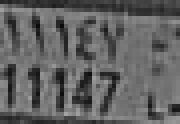
\includegraphics[width=0.9\linewidth]{../assets/plate_gray.png}\\{\scriptsize original}\\[4pt]
      
\includegraphics[width=0.9\linewidth]{../assets/plate_sharp.png}\\{\scriptsize unsharp-masked}
    \end{center}\end{column}
    \begin{column}{0.5\textwidth}
      \begin{itemize}
        \item \term{Unsharp mask}: $\text{sharp} = \text{img} + \lambda(\text{img}-\text{blur})$.
        \item The $(\text{img}-\text{blur})$ term \emph{is} the high-frequency detail.
        \item Adds it back to emphasize edges — the digits' strokes stand out.
      \end{itemize}
    \end{column}
  \end{columns}
\end{frame}

\begin{frame}{Why ``unsharp'' means sharpen}
  \begin{mathbox}[The detail signal]
    $\text{detail} = \text{img} - \text{blur}(\text{img})$\qquad
    $\text{sharp} = \text{img} + \lambda\cdot\text{detail}$
  \end{mathbox}
  \begin{itemize}
    \item Subtracting a blurred (``unsharp'') copy leaves only what the blur removed — the fine detail.
    \item Add a scaled copy of that detail back and edges get exaggerated.
    \item $\lambda$ is the strength: $\lambda=1$ is moderate; $\lambda=3$ is aggressive.
  \end{itemize}
  \keyidea{The name is historical (a darkroom trick); the math is just image $+$ its own high-pass.}
\end{frame}

\begin{frame}{The sharpen kernel is unsharp mask in one step}
  \begin{columns}[T]
    \begin{column}{0.5\textwidth}
      Combine identity and (identity $-$ box) into a single kernel:
      \[
      \underbrace{\begin{bmatrix}0&0&0\\0&1&0\\0&0&0\end{bmatrix}}_{\text{identity}}
      +\lambda\Big(\text{id}-\text{blur}\Big)
      =\begin{bmatrix}0&-1&0\\-1&5&-1\\0&-1&0\end{bmatrix}
      \]
    \end{column}
    \begin{column}{0.5\textwidth}
      \begin{itemize}
        \item Centre $5$ = the pixel plus its own boosted detail.
        \item Sides $-1$ = subtract the neighbours (the local average).
        \item Sums to $1$ $\Rightarrow$ flat regions unchanged, only edges pop.
      \end{itemize}
    \end{column}
  \end{columns}
  \begin{infobox}
    A single convolution does the whole unsharp mask when the blur is a small box — no separate subtract step.
  \end{infobox}
\end{frame}

\begin{frame}[fragile]{\faPen~Warm-up exercise (8 min)}
  \begin{infobox}[Sharpen by hand]
  \end{infobox}
  A patch with an edge (dark left, bright right) and the sharpen kernel:
  \[
  P=\begin{bmatrix}10&10&200\\10&10&200\\10&10&200\end{bmatrix}\qquad
  K=\begin{bmatrix}0&-1&0\\-1&5&-1\\0&-1&0\end{bmatrix}
  \]
  \begin{enumerate}
    \item Compute the output at the centre pixel (value $10$, its right neighbour is $200$).
    \item Is the result pulled toward the dark side or the bright side? What does that do at an edge?
  \end{enumerate}
\end{frame}

\begin{frame}{\faPen~Debrief}
  \begin{itemize}
    \item Centre: $5(10) - 10 - 10 - 10 - 200 = 50 - 230 = \mathbf{-180}$, clamped to $\mathbf{0}$.
    \item The dark side of the edge is driven \emph{darker} (to 0); by symmetry the bright side is driven brighter.
    \item That widening gap is exactly the bright/dark rim you see along a sharpened edge — enhanced local contrast.
  \end{itemize}
  \keyidea{Sharpening pushes the two sides of an edge apart. Push too hard and the rim becomes a visible halo.}
\end{frame}

\begin{frame}{High-boost \& the Laplacian}
  \begin{columns}[T]
    \begin{column}{0.5\textwidth}
      \term{High-boost} generalizes the centre weight:
      \[
      \begin{bmatrix}0&-1&0\\-1&\,A{+}4\,&-1\\0&-1&0\end{bmatrix}
      \]
      $A=1$ is the plain sharpen; larger $A$ keeps more of the original.
    \end{column}
    \begin{column}{0.5\textwidth}
      The \term{Laplacian} is the pure high-pass ($\sum=0$):
      \[
      \begin{bmatrix}0&-1&0\\-1&4&-1\\0&-1&0\end{bmatrix}
      \]
      Sharpen $=$ image $+$ Laplacian. It measures how much a pixel differs from its surround.
    \end{column}
  \end{columns}
  \begin{infobox}
    Same family, one knob: sharpen, high-boost and Laplacian differ only in the centre weight.
  \end{infobox}
\end{frame}

\begin{frame}{Sharpening's catch}
  \begin{itemize}
    \item It amplifies \emph{everything} high-frequency — including noise and JPEG blocks.
    \item Over-sharpening creates \term{halos} (bright/dark rings) around edges.
    \item Denoise first, then sharpen gently. Never sharpen a noisy image blindly.
  \end{itemize}
  \begin{badbox}
    Sharpening a raw, noisy meter crop turns sensor speckle into a field of bright dots that
    wrecks the threshold. Smooth (Session 1) \emph{then} sharpen.
  \end{badbox}
  \keyidea{Blur and sharpen are opposites, but they're both convolution — just different kernels.}
\end{frame}

% ==================================================================
\section{Nonlinear filters}
% ==================================================================

\begin{frame}{Nonlinear filter: the median}
  \begin{columns}[T]
    \begin{column}{0.5\textwidth}\begin{center}
      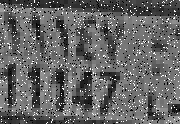
\includegraphics[width=0.85\linewidth]{../assets/plate_noisy.png}\\{\scriptsize salt-and-pepper noise}\\[3pt]
      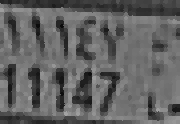
\includegraphics[width=0.85\linewidth]{../assets/plate_median.png}\\{\scriptsize 3$\times$3 median}
    \end{center}\end{column}
    \begin{column}{0.5\textwidth}
      \begin{itemize}
        \item A \term{median} filter takes the median of the neighbourhood — not a weighted sum.
        \item It kills salt-and-pepper noise while keeping edges sharp (a Gaussian would smear them).
        \item Nonlinear $\rightarrow$ not convolution, but same ``slide a window'' idea.
      \end{itemize}
    \end{column}
  \end{columns}
\end{frame}

\begin{frame}{Why the median beats the mean on spikes}
  \begin{columns}[T]
    \begin{column}{0.52\textwidth}
      Neighbourhood values (one ``salt'' spike):
      \[ \{12,\,14,\,13,\,\mathbf{255},\,15,\,13,\,14,\,12,\,15\} \]
      \begin{itemize}
        \item \term{Mean} $=40.3$ — the spike dragged it up.
        \item \term{Median} (sorted, middle) $=14$ — the spike is simply \emph{discarded}.
      \end{itemize}
    \end{column}
    \begin{column}{0.48\textwidth}
      \begin{goodbox}
        The median is an \term{order statistic}: one wild outlier cannot move it, because it
        never enters the arithmetic — it just sits at the end of the sorted list.
      \end{goodbox}
    \end{column}
  \end{columns}
  \keyidea{Mean averages the outlier in; median throws it out. That is why median wins on impulsive noise.}
\end{frame}

\begin{frame}{The rank-filter family}
  \begin{columns}[T]
    \begin{column}{0.55\textwidth}
      Sort the neighbourhood, then pick a position:
      \begin{itemize}
        \item \term{min} filter (erosion-like): darkens, removes bright specks.
        \item \term{max} filter (dilation-like): brightens, removes dark specks.
        \item \term{median}: the middle — balanced impulse removal.
      \end{itemize}
    \end{column}
    \begin{column}{0.45\textwidth}
      \begin{center}
      \pixelgrid{ {12,14,13}, {15,255,13}, {14,12,15} }\\[3pt]
      {\scriptsize sorted: 12,12,13,13,\textbf{14},15,15,\dots,255}
      \end{center}
    \end{column}
  \end{columns}
  \begin{infobox}
    Min/max are the seed of \term{morphology} (Week 4). Median sits between them and is the
    workhorse for salt-and-pepper.
  \end{infobox}
\end{frame}

\begin{frame}{Bilateral filter: smooth but keep edges}
  \begin{itemize}
    \item Gaussian blur smears edges; the \term{bilateral} filter weights by \emph{both} distance \emph{and} intensity similarity.
    \item Result: flat regions get smoothed, edges stay crisp — great before thresholding a document.
    \item Slower, but often the right smoother for DocScan: \code{cv2.bilateralFilter}.
  \end{itemize}
  \begin{mathbox}
    $w(i,j)=\underbrace{e^{-\frac{i^2+j^2}{2\sigma_s^2}}}_{\text{spatial}}\;
             \underbrace{e^{-\frac{(f_p-f_q)^2}{2\sigma_r^2}}}_{\text{range}}$
  \end{mathbox}
  \begin{goodbox}
    When you need to denoise \emph{without} blurring the digit edges, reach for bilateral (or median).
  \end{goodbox}
\end{frame}

\begin{frame}{Tuning the bilateral filter}
  \begin{columns}[T]
    \begin{column}{0.55\textwidth}
      \begin{itemize}
        \item \term{$\sigma_s$} (spatial): how far a neighbour can be and still count — like a Gaussian radius.
        \item \term{$\sigma_r$} (range): how different in intensity a neighbour can be and still count.
        \item Large $\sigma_r$ $\rightarrow$ behaves like a plain Gaussian (edges start to smear again).
        \item Small $\sigma_r$ $\rightarrow$ only near-equal pixels mix, so edges are strongly preserved.
      \end{itemize}
    \end{column}
    \begin{column}{0.45\textwidth}
      \begin{badbox}
        It is expensive: cost grows with window size and it is not separable. Don't run it on a
        full frame every loop iteration — crop to the region of interest first.
      \end{badbox}
    \end{column}
  \end{columns}
  \keyidea{$\sigma_r$ is the ``edge sensitivity'' knob — the whole reason to prefer bilateral over Gaussian.}
\end{frame}

\begin{frame}{A zoo of kernels \& filters}
  \begin{center}
  \begin{tabular}{@{}lll@{}}
    \toprule
    \textbf{Filter} & \textbf{Effect} & \textbf{Linear?} \\
    \midrule
    all $1/n$ & box blur (average) & yes \\
    Gaussian weights & smooth blur & yes \\
    centre 5, sides $-1$ & sharpen (high-pass) & yes \\
    $[-1,0,1]$ rows & horizontal gradient (edges, Week 5) & yes \\
    identity + (id $-$ blur) & unsharp mask & yes \\
    median of window & impulse-noise removal & no \\
    bilateral & edge-preserving smooth & no \\
    \bottomrule
  \end{tabular}
  \end{center}
  \keyidea{You don't memorize kernels — you understand what ``average'' vs ``difference'' vs ``order statistic'' does.}
\end{frame}

% ==================================================================
\section{Deep dive}
% ==================================================================

\begin{frame}{Frequency view: low-pass vs high-pass}
  \begin{columns}[T]
    \begin{column}{0.58\textwidth}
      \begin{itemize}
        \item Smoothing keeps \term{low frequencies} (slow changes), removes high (a \term{low-pass} filter).
        \item Sharpening/edges keep \term{high frequencies} (fast changes) — a \term{high-pass} filter.
        \item Week 6 makes this literal with the Fourier transform; today it's intuition.
      \end{itemize}
    \end{column}
    \begin{column}{0.42\textwidth}
      \begin{center}
      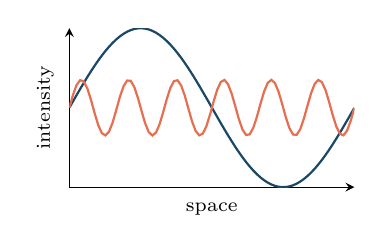
\begin{tikzpicture}[font=\scriptsize]
        \begin{axis}[width=5.2cm,height=3.6cm,domain=0:6.28,samples=80,
          axis lines=left,xtick=\empty,ytick=\empty,
          xlabel={space},ylabel={intensity}]
          \addplot[coursePrimary,thick]{sin(deg(x))};
          \addplot[courseAccent,thick]{0.35*sin(deg(6*x))};
        \end{axis}
      \end{tikzpicture}\\
      {\scriptsize blue = low freq (kept by blur)\\ coral = high freq (kept by sharpen)}
      \end{center}
    \end{column}
  \end{columns}
  \begin{goodbox}
    ``Blur = low-pass, edges = high-pass'' is a lens you'll use for the rest of the course.
  \end{goodbox}
\end{frame}

\begin{frame}{Separability \& speed}
  \begin{columns}[T]
    \begin{column}{0.55\textwidth}
      \begin{itemize}
        \item A separable 2D kernel = outer product of two 1D kernels; apply them in sequence.
        \item A $k\times k$ blur costs $k^2$ multiplies per pixel; separated, only $2k$.
        \item OpenCV does this automatically for Gaussian; know it so you write fast filters.
      \end{itemize}
    \end{column}
    \begin{column}{0.45\textwidth}
      \begin{mathbox}[Cost, $k=9$]
        naive: $k^2 = 81$/pixel\\
        separated: $2k = 18$/pixel\\[2pt]
        $\Rightarrow 4.5\times$ faster, and it grows with $k$.
      \end{mathbox}
    \end{column}
  \end{columns}
  \begin{infobox}
    The $3\times3$ Gaussian $\tfrac{1}{16}[1,2,1;2,4,2;1,2,1]$ is $\tfrac14[1,2,1]$ applied
    horizontally then vertically — proof by construction.
  \end{infobox}
\end{frame}

\begin{frame}{Convolution is the bridge to deep learning}
  \begin{itemize}
    \item A CNN layer (Week 13) is exactly this: convolve the image with small kernels.
    \item The difference: the network \emph{learns} the kernel values from data instead of you designing them.
    \item Everything you learn about kernels this week is what a CNN's first layers do.
  \end{itemize}
  \keyidea{Classical filters are hand-designed kernels; CNNs are learned kernels. Same operation.}
\end{frame}

\begin{frame}[fragile]{Filtering in code — the full toolbox}
\begin{lstlisting}[language=Python]
box    = cv2.blur(img, (5, 5))
gauss  = cv2.GaussianBlur(img, (7, 7), 1.5)
median = cv2.medianBlur(img, 3)             # nonlinear, impulse noise
bilat  = cv2.bilateralFilter(img, 9, 75, 75)# edge-preserving smooth
k = np.array([[0,-1,0],[-1,5,-1],[0,-1,0]])
sharp  = cv2.filter2D(img, -1, k)           # any custom kernel
\end{lstlisting}
  \code{cv2.filter2D} convolves with any kernel you give it — the general tool the others are shortcuts for.
\end{frame}

\begin{frame}{Which filter, when? — a decision guide}
  \begin{center}
  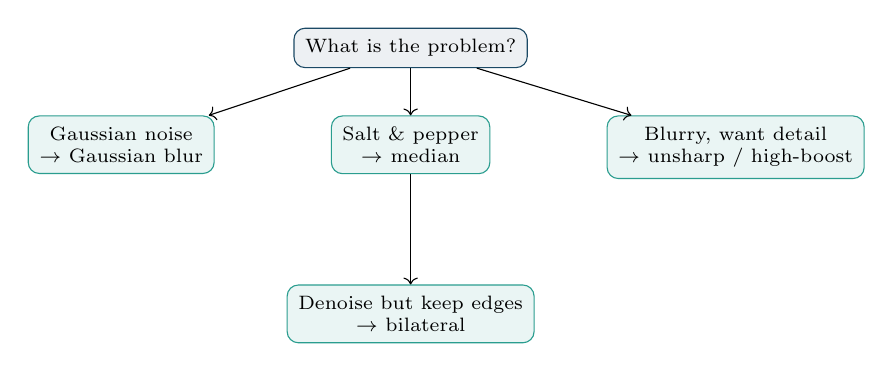
\begin{tikzpicture}[font=\scriptsize,node distance=6mm and 10mm,
      box/.style={draw=coursePrimary,rounded corners,fill=coursePrimary!8,align=center,inner sep=4pt},
      leaf/.style={draw=courseGood,rounded corners,fill=courseGood!10,align=center,inner sep=4pt}]
    \node[box] (q1) {What is the problem?};
    \node[leaf,below left=of q1] (a) {Gaussian noise\\$\rightarrow$ Gaussian blur};
    \node[leaf,below=of q1] (b) {Salt \& pepper\\$\rightarrow$ median};
    \node[leaf,below right=of q1] (c) {Blurry, want detail\\$\rightarrow$ unsharp / high-boost};
    \node[leaf,below=14mm of b] (d) {Denoise but keep edges\\$\rightarrow$ bilateral};
    \draw[->] (q1)--(a); \draw[->] (q1)--(b); \draw[->] (q1)--(c); \draw[->] (b)--(d);
  \end{tikzpicture}
  \end{center}
  \keyidea{Match the filter to the \emph{noise/goal}, not to habit. The zoo exists because no one filter wins everywhere.}
\end{frame}

\begin{frame}{Common pitfalls, collected}
  \begin{badbox}[Sharpen-then-notice-the-noise]
    Sharpening amplifies noise. Always denoise \emph{first}, then sharpen gently.
  \end{badbox}
  \begin{badbox}[Median for the wrong noise]
    Median is superb for impulse noise but poor for fine Gaussian grain — use Gaussian/bilateral there.
  \end{badbox}
  \begin{badbox}[Over-blur before threshold]
    Enough blur to kill noise, not so much the digit strokes merge — tune $\sigma$ on your own images.
  \end{badbox}
\end{frame}

\begin{frame}{Linear vs nonlinear: what you keep or lose}
  \begin{center}
  \begin{tabular}{@{}lcc@{}}
    \toprule
    & \textbf{Linear (convolution)} & \textbf{Nonlinear (median/bilateral)} \\
    \midrule
    Separable / very fast & often yes & no \\
    Superposition holds & yes & no \\
    Edge preservation & poor (blur) & good \\
    Impulse-noise removal & poor & excellent \\
    Analyzable in frequency & yes (Week 6) & not directly \\
    \bottomrule
  \end{tabular}
  \end{center}
  \keyidea{Linear filters are fast and analyzable; nonlinear ones protect edges. Pick the property you need.}
\end{frame}

% ==================================================================
\section{Wrap-up}
% ==================================================================

\begin{frame}{Putting it together: the DocScan pre-filter chain}
  \begin{center}
  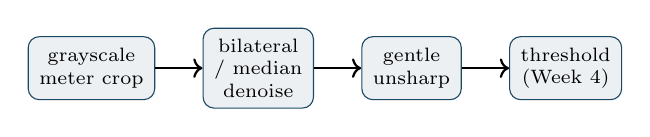
\begin{tikzpicture}[font=\scriptsize,node distance=6mm,
      s/.style={draw=coursePrimary,rounded corners,fill=coursePrimary!8,align=center,inner sep=4pt,minimum height=8mm}]
    \node[s] (a) {grayscale\\meter crop};
    \node[s,right=of a] (b) {bilateral\\/ median\\denoise};
    \node[s,right=of b] (c) {gentle\\unsharp};
    \node[s,right=of c] (d) {threshold\\(Week 4)};
    \draw[->,thick] (a)--(b); \draw[->,thick] (b)--(c); \draw[->,thick] (c)--(d);
  \end{tikzpicture}
  \end{center}
  \begin{itemize}
    \item Denoise with an \emph{edge-preserving} filter so the digit strokes survive.
    \item A light sharpen recovers stroke contrast the denoise softened.
    \item Only then threshold — a clean, sharp mask is far easier to read.
  \end{itemize}
  \keyidea{Filters are rarely used alone; they form a short pipeline tuned to your images.}
\end{frame}

\begin{frame}{What you should now be able to do}
  \begin{itemize}
    \item Sharpen with the unsharp mask, derive its kernel, and predict the halos it causes.
    \item Choose between mean, median and bilateral for a given kind of noise.
    \item See the low-pass/high-pass view and exploit separability for speed.
    \item Connect classical kernels to the learned kernels of a CNN.
  \end{itemize}
\end{frame}

\begin{frame}{This week's deliverable}
  \begin{alertblock}{Due before Week 4 (see \code{project/})}
    On real meter/plate images:
    \begin{enumerate}
      \item Implement a 3$\times$3 convolution \emph{from scratch} (NumPy, Session 1) and match \code{cv2.filter2D}.
      \item Compare box vs Gaussian blur at several sizes; discuss detail loss vs noise removal.
      \item Sharpen a plate with unsharp mask; find where it starts creating halos.
      \item Add salt-and-pepper noise and compare median vs Gaussian denoising.
      \item Note: what blur helps your DocScan threshold, and what over-blurs the digits?
    \end{enumerate}
  \end{alertblock}
\end{frame}

\begin{frame}[standout]
  The kernel is the algorithm.\\[4pt]
  \normalsize Blur, sharpen, edges — all the same operation with different numbers.
\end{frame}

\end{document}
